\chapter{Representing a Game}

Typically we have two ways to represent a game:
\begin{itemize}
  \item Extensive form (game tree)
  \item Normal form (payoff matrix)
\end{itemize}

\section{Game Tree}
\ex[Chess]{
  \begin{minipage}{0.48\textwidth}
\centering
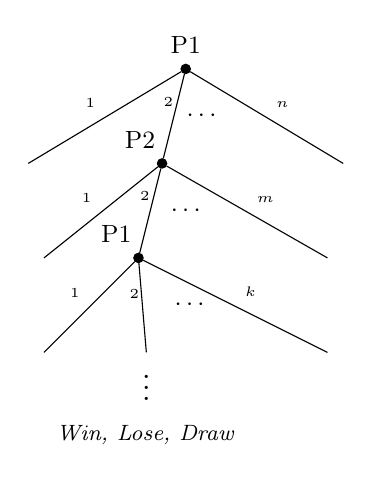
\begin{tikzpicture}[scale=1, font=\small]
    % Node styles
    \tikzset{solid node/.style={circle,draw,fill=black,inner sep=1.2pt}}
    
    % Root node - Player 1
    \node[solid node, label=above:P1] (root) at (0, 0) {};
    
    % Level 1: branches from Player 1
    \coordinate (b1) at (-2, -1.2);
    \coordinate (b4) at (2, -1.2);
    
    % Level 2 - Player 2 node (tilted left)
    \node[solid node, label={[xshift=-8pt]above:P2}] (p2) at (-0.3, -1.2) {};
    
    % Draw lines from Player 1
    \draw (root) -- (b1) node[midway, above left, font=\tiny] {1};
    \draw (root) -- (p2) node[midway, above, font=\tiny, xshift=-2pt] {2};
    \node at (0.2, -0.6) {\small $\cdots$};
    \draw (root) -- (b4) node[midway, above right, font=\tiny] {$n$};
    
    % Level 2: branches from Player 2
    \coordinate (c1) at (-1.8, -2.4);
    \coordinate (c4) at (1.8, -2.4);
    
    % Level 3 - Player 1 node (tilted left)
    \node[solid node, label={[xshift=-8pt]above:P1}] (p1_2) at (-0.6, -2.4) {};
    
    % Draw lines from Player 2
    \draw (p2) -- (c1) node[midway, above left, font=\tiny] {1};
    \draw (p2) -- (p1_2) node[midway, above, font=\tiny, xshift=-2pt] {2};
    \node at (0, -1.8) {\small $\cdots$};
    \draw (p2) -- (c4) node[midway, above right, font=\tiny] {$m$};
    
    % Level 3: branches from Player 1
    \coordinate (d1) at (-1.8, -3.6);
    \coordinate (d2) at (-0.5, -3.6);
    \coordinate (d4) at (1.8, -3.6);
    
    % Draw lines from Player 1 (second decision node)
    \draw (p1_2) -- (d1) node[midway, above left, font=\tiny] {1};
    \draw (p1_2) -- (d2) node[midway, above, font=\tiny, xshift=-3pt] {2};
    \node at (0.05, -3) {\small $\cdots$};
    \draw (p1_2) -- (d4) node[midway, above right, font=\tiny] {$k$};
    
    % Vertical ellipsis and outcomes
    \node at (-0.5, -3.95) {\large $\vdots$};
    \node at (-0.5, -4.65) {\footnotesize \textit{Win, Lose, Draw}};
\end{tikzpicture}
\end{minipage}%
\hspace{0.02\textwidth}
\begin{minipage}{0.48\textwidth}
\centering
$\begin{cases}
  \text{Nodes} \\[6pt]
  \text{Players} \\[6pt]
  \text{Choices at every node} \\[6pt]
  \text{Terminal nodes (outcome)} \\[6pt]
  \text{Information sets}
\end{cases}$
\end{minipage}
}

\defn{Game with Perfect / Imperfect Information}{
  \begin{itemize}
    \item A game with perfect information is a game where a player at node $n$ knows all the moves that lead to $n$.
    \item A game with imperfect information is a game where a player at node $n$ only knows some moves that lead to $n$.
  \end{itemize}
}

\ex[Matching Pennies]{
\begin{center}
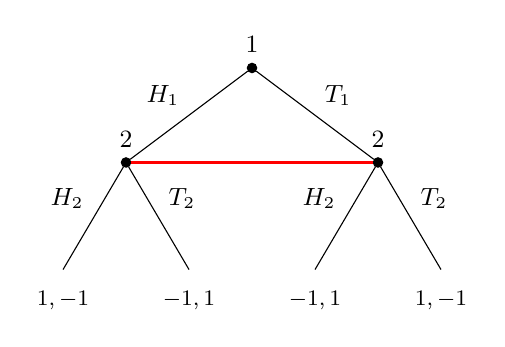
\begin{tikzpicture}[scale=0.8, font=\small]
    % Node styles
    \tikzset{solid node/.style={circle,draw,fill=black,inner sep=1.2pt}}
    
    % Root node - Player 1
    \node[solid node, label=above:1] (root) at (0, 0) {};
    
    % Level 1: branches from Player 1 (H and T choices)
    \coordinate (h) at (-2, -1.5);
    \coordinate (t) at (2, -1.5);
    
    % Level 2 - Player 2 nodes
    \node[solid node, label=above:2] (p2_h) at (-2, -1.5) {};
    \node[solid node, label=above:2] (p2_t) at (2, -1.5) {};
    
    % Draw lines from Player 1
    \draw (root) -- (p2_h) node[midway, above left, font=\small] {$H_1$};
    \draw (root) -- (p2_t) node[midway, above right, font=\small] {$T_1$};
    
    % Information Set for Player 2 (red line connecting the two nodes)
    \draw[red, thick] (p2_h) -- (p2_t);
    
    % Level 3: terminal nodes
    \coordinate (hh) at (-3, -3.2);
    \coordinate (ht) at (-1, -3.2);
    \coordinate (th) at (1, -3.2);
    \coordinate (tt) at (3, -3.2);
    
    % Draw lines from Player 2 nodes
    \draw (p2_h) -- (hh) node[midway, above left, font=\small] {$H_2$};
    \draw (p2_h) -- (ht) node[midway, above right, font=\small] {$T_2$};
    \draw (p2_t) -- (th) node[midway, above left, font=\small] {$H_2$};
    \draw (p2_t) -- (tt) node[midway, above right, font=\small] {$T_2$};
    
    % Terminal outcomes
    \node at (hh) [below=0.15cm] {\footnotesize $1, -1$};
    \node at (ht) [below=0.15cm] {\footnotesize $-1, 1$};
    \node at (th) [below=0.15cm] {\footnotesize $-1, 1$};
    \node at (tt) [below=0.15cm] {\footnotesize $1, -1$};
\end{tikzpicture}
\end{center}
}

\section{Information Sets}

All the nodes of a game tree are partitioned into information sets.

\state{Rules for Information Sets}{
  \begin{itemize}
  \item Each node in an information set must belong to the same player.
  \item Each node in an information set must have the same choices.
\end{itemize}
}

\ex[]{
  \begin{minipage}{0.48\textwidth}
    \centering
    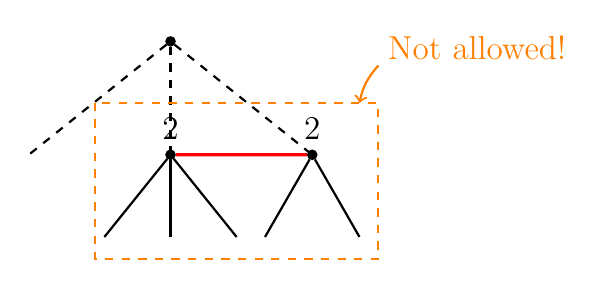
\begin{tikzpicture}[scale=1.2, font=\large]
      \tikzset{solid node/.style={circle,draw,fill=black,inner sep=1.2pt}}
      
      % Root node
      \node[solid node] (root) at (0, 0) {};
      
      % Three dashed branches from root
      \draw[dashed, thick] (root) -- (0, -1.2);
      \draw[dashed, thick] (root) -- (-1.5, -1.2);
      \draw[dashed, thick] (root) -- (1.5, -1.2);
      
      % Middle node with label 2
      \node[solid node, label=above:2] (n2_mid) at (0, -1.2) {};
      
      % Right node with label 2
      \node[solid node, label=above:2] (n2_right) at (1.5, -1.2) {};
      
      % From middle node 2 - three branches
      \draw[thick] (n2_mid) -- (-0.7, -2.07);
      \draw[thick] (n2_mid) -- (0, -2.07);
      \draw[thick] (n2_mid) -- (0.7, -2.07);
      
      % From right node 2 - two branches on the right
      \draw[thick] (n2_right) -- (1, -2.07);
      \draw[thick] (n2_right) -- (2, -2.07);
      
      % Red information set connecting the two 2s
      \draw[red, very thick] (n2_mid) -- (n2_right);
      
      % --- Dotted box around problematic structure ---
      \draw[orange, thick, dashed] (-0.8, -0.65) rectangle (2.2, -2.3);
      
      % "Not allowed!" annotation for first tree
      \node[orange, font=\large, anchor=south west] (msg1) at (2.2, -0.3) {Not allowed!};
      \draw[->, orange, thick] (msg1) to[bend right=15] (2.0, -0.65);
      
    \end{tikzpicture}
  \end{minipage}%
  \hspace{0.02\textwidth}
  \begin{minipage}{0.48\textwidth}
    \centering
    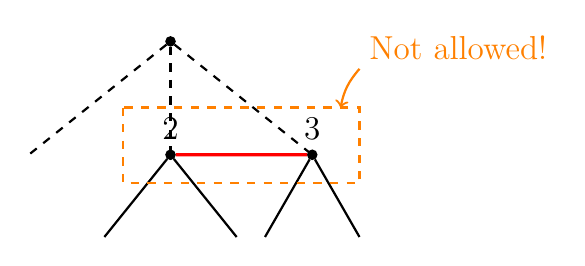
\begin{tikzpicture}[scale=1.2, font=\large]
      \tikzset{solid node/.style={circle,draw,fill=black,inner sep=1.2pt}}
      
      % Root node
      \node[solid node] (root) at (0, 0) {};
      
      % Three dashed branches from root
      \draw[dashed, thick] (root) -- (0, -1.2);
      \draw[dashed, thick] (root) -- (-1.5, -1.2);
      \draw[dashed, thick] (root) -- (1.5, -1.2);
      
      % Middle node with label 2
      \node[solid node, label=above:2] (n2) at (0, -1.2) {};
      
      % Right node with label 3
      \node[solid node, label=above:3] (n3) at (1.5, -1.2) {};
      
      % From node 2 - three branches
      \draw[thick] (n2) -- (-0.7, -2.07);
      \draw[thick] (n2) -- (0.7, -2.07);
      
      % From node 3 - two branches on the right
      \draw[thick] (n3) -- (1, -2.07);
      \draw[thick] (n3) -- (2, -2.07);
      
      % Red information set connecting 2 and 3
      \draw[red, very thick] (n2) -- (n3);
      
      % --- Dotted box around problematic structure ---
      \draw[orange, thick, dashed] (-0.5, -0.7) rectangle (2, -1.5);
      
      % "Not allowed!" annotation for second tree
      \node[orange, font=\large, anchor=south west] (msg2) at (2.0, -0.3) {Not allowed!};
      \draw[->, orange, thick] (msg2) to[bend right=15] (1.8, -0.7);
      
    \end{tikzpicture}
  \end{minipage}
  \\\par
  The first tree is invalid because the two nodes in the information set have different choices. The second tree is invalid because the two nodes in the information set belong to different players.
}

\ex[Coin Toss Revisited]{
\noindent
\begin{minipage}{0.45\textwidth}
\centering
\textbf{Cointoss Not Revealed to Player 1}
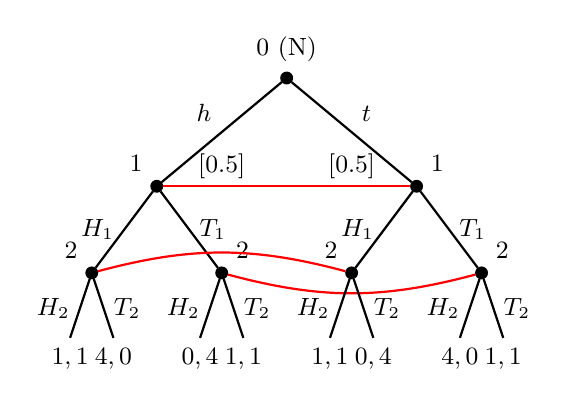
\begin{tikzpicture}[scale=0.55, font=\small]
    % Node style
    \tikzstyle{solid node}=[circle,draw,inner sep=1.5pt,fill=black]
    \tikzstyle{hollow node}=[circle,draw,inner sep=1.5pt]

    % --- Level 0: Nature ---
    \node[solid node, label=above:{0 (N)}] (root) at (0,1) {};

    % --- Level 1: Player 1 ---
    % Positions
    \node[solid node, label=above left:1] (n1_left) at (-3, -1.5) {};
    \node[solid node, label=above right:1] (n1_right) at (3, -1.5) {};

    % Edges from Nature
    \draw[thick] (root) -- node[above left] {$h$} node[below=4pt] {[0.5]} (n1_left);
    \draw[thick] (root) -- node[above right] {$t$} node[below=4pt] {[0.5]} (n1_right);

    % Information Set for Player 1 (Red Line)
    \draw[red, thick] (n1_left) -- (n1_right);

    % --- Level 2: Player 2 ---
    \node[solid node, label=above left:2] (n2_1) at (-4.5, -3.5) {}; % h -> H1
    \node[solid node, label=above right:2] (n2_2) at (-1.5, -3.5) {}; % h -> T1
    
    % From Right Node (t)
    \node[solid node, label=above left:2] (n2_3) at (1.5, -3.5) {};  % t -> H1
    \node[solid node, label=above right:2] (n2_4) at (4.5, -3.5) {};  % t -> T1

    % Edges from Player 1
    \draw[thick] (n1_left) -- node[left] {$H_1$} (n2_1);
    \draw[thick] (n1_left) -- node[right] {$T_1$} (n2_2);
    \draw[thick] (n1_right) -- node[left] {$H_1$} (n2_3);
    \draw[thick] (n1_right) -- node[right] {$T_1$} (n2_4);

    % Information Sets for Player 2 (Curved Red Lines)
    % Connects "Heard H1" nodes (n2_1 and n2_3)
    \draw[red, thick] (n2_1) to[bend left=15] (n2_3);
    
    % Connects "Heard T1" nodes (n2_2 and n2_4)
    \draw[red, thick] (n2_2) to[bend right=15] (n2_4);

    % --- Level 3: Leaves and Payoffs ---
    % Helper coordinates for leaves
    % h -> H1 -> ...
    \coordinate (l_1) at (-5.0, -5);
    \coordinate (l_2) at (-4.0, -5);
    
    % h -> T1 -> ...
    \coordinate (l_3) at (-2.0, -5);
    \coordinate (l_4) at (-1.0, -5);

    % t -> H1 -> ...
    \coordinate (l_5) at (1.0, -5);
    \coordinate (l_6) at (2.0, -5);

    % t -> T1 -> ...
    \coordinate (l_7) at (4.0, -5);
    \coordinate (l_8) at (5.0, -5);

    % Drawing Edges and Payoffs
    % Branch 1 (h -> H1)
    \draw[thick] (n2_1) -- node[left] {$H_2$} (l_1) node[below] {$1,1$};
    \draw[thick] (n2_1) -- node[right] {$T_2$} (l_2) node[below] {$4,0$};

    % Branch 2 (h -> T1)
    \draw[thick] (n2_2) -- node[left] {$H_2$} (l_3) node[below] {$0,4$};
    \draw[thick] (n2_2) -- node[right] {$T_2$} (l_4) node[below] {$1,1$};

    % Branch 3 (t -> H1)
    \draw[thick] (n2_3) -- node[left] {$H_2$} (l_5) node[below] {$1,1$};
    \draw[thick] (n2_3) -- node[right] {$T_2$} (l_6) node[below] {$0,4$};

    % Branch 4 (t -> T1)
    \draw[thick] (n2_4) -- node[left] {$H_2$} (l_7) node[below] {$4,0$};
    \draw[thick] (n2_4) -- node[right] {$T_2$} (l_8) node[below] {$1,1$};

\end{tikzpicture}
\end{minipage}%
\hspace{0.02\textwidth}
\begin{minipage}{0.45\textwidth}
\centering
\textbf{Cointoss Revealed to Player 1}
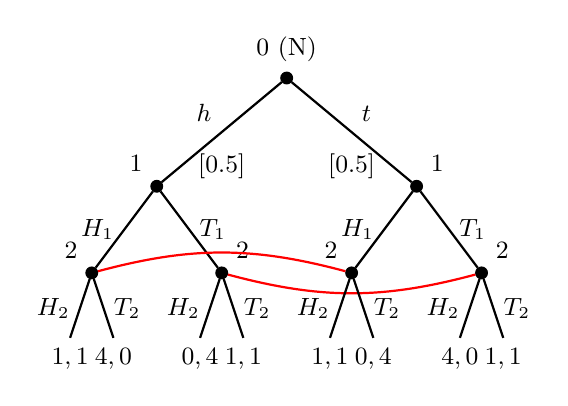
\begin{tikzpicture}[scale=0.55, font=\small]
    % Node style
    \tikzstyle{solid node}=[circle,draw,inner sep=1.5pt,fill=black]
    \tikzstyle{hollow node}=[circle,draw,inner sep=1.5pt]

    % --- Level 0: Nature ---
    \node[solid node, label=above:{0 (N)}] (root) at (0,1) {};

    % --- Level 1: Player 1 ---
    % Positions
    \node[solid node, label=above left:1] (n1_left) at (-3, -1.5) {};
    \node[solid node, label=above right:1] (n1_right) at (3, -1.5) {};

    % Edges from Nature
    \draw[thick] (root) -- node[above left] {$h$} node[below=4pt] {[0.5]} (n1_left);
    \draw[thick] (root) -- node[above right] {$t$} node[below=4pt] {[0.5]} (n1_right);

    % --- Level 2: Player 2 ---
    % Positions (Spread out to fit the tree)
    % From Left Node (h)
    \node[solid node, label=above left:2] (n2_1) at (-4.5, -3.5) {}; % h -> H1
    \node[solid node, label=above right:2] (n2_2) at (-1.5, -3.5) {}; % h -> T1
    
    % From Right Node (t)
    \node[solid node, label=above left:2] (n2_3) at (1.5, -3.5) {};  % t -> H1
    \node[solid node, label=above right:2] (n2_4) at (4.5, -3.5) {};  % t -> T1

    % Edges from Player 1
    \draw[thick] (n1_left) -- node[left] {$H_1$} (n2_1);
    \draw[thick] (n1_left) -- node[right] {$T_1$} (n2_2);
    \draw[thick] (n1_right) -- node[left] {$H_1$} (n2_3);
    \draw[thick] (n1_right) -- node[right] {$T_1$} (n2_4);

    % Information Sets for Player 2 (Curved Red Lines)
    % Connects "Heard H1" nodes (n2_1 and n2_3)
    \draw[red, thick] (n2_1) to[bend left=15] (n2_3);
    
    % Connects "Heard T1" nodes (n2_2 and n2_4)
    \draw[red, thick] (n2_2) to[bend right=15] (n2_4);

    % --- Level 3: Leaves and Payoffs ---
    % Helper coordinates for leaves
    % h -> H1 -> ...
    \coordinate (l_1) at (-5.0, -5);
    \coordinate (l_2) at (-4.0, -5);
    
    % h -> T1 -> ...
    \coordinate (l_3) at (-2.0, -5);
    \coordinate (l_4) at (-1.0, -5);

    % t -> H1 -> ...
    \coordinate (l_5) at (1.0, -5);
    \coordinate (l_6) at (2.0, -5);

    % t -> T1 -> ...
    \coordinate (l_7) at (4.0, -5);
    \coordinate (l_8) at (5.0, -5);

    % Drawing Edges and Payoffs
    % Branch 1 (h -> H1)
    \draw[thick] (n2_1) -- node[left] {$H_2$} (l_1) node[below] {$1,1$};
    \draw[thick] (n2_1) -- node[right] {$T_2$} (l_2) node[below] {$4,0$};

    % Branch 2 (h -> T1)
    \draw[thick] (n2_2) -- node[left] {$H_2$} (l_3) node[below] {$0,4$};
    \draw[thick] (n2_2) -- node[right] {$T_2$} (l_4) node[below] {$1,1$};

    % Branch 3 (t -> H1)
    \draw[thick] (n2_3) -- node[left] {$H_2$} (l_5) node[below] {$1,1$};
    \draw[thick] (n2_3) -- node[right] {$T_2$} (l_6) node[below] {$0,4$};

    % Branch 4 (t -> T1)
    \draw[thick] (n2_4) -- node[left] {$H_2$} (l_7) node[below] {$4,0$};
    \draw[thick] (n2_4) -- node[right] {$T_2$} (l_8) node[below] {$1,1$};

\end{tikzpicture}
\end{minipage}
}

\asm{}{
Each path from the root to a terminal node intersects each information set at most once.
}

\ex[Absent-Minded Driver]{
  \par\centering
  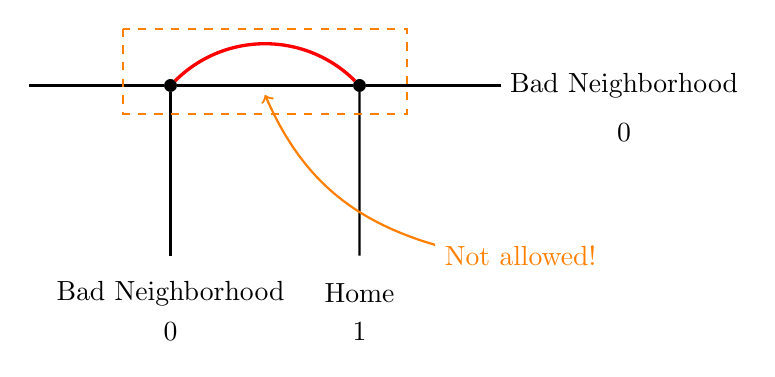
\begin{tikzpicture}[scale=1.2]
    % Node styles
    \tikzset{solid node/.style={circle,draw,fill=black,inner sep=1.5pt}}
    
    % --- Decision nodes on horizontal line ---
    \node[solid node] (n1) at (0, 0) {};
    \node[solid node] (n2) at (2, 0) {};
    
    % --- Horizontal branches ---
    \draw[thick] (-1.5, 0) -- (n1);  % From left to n1
    \draw[thick] (n1) -- (n2);  % Between n1 and n2
    \draw[thick] (n2) -- (3.5, 0);  % From n2 to right exit
    
    % --- Vertical branch from n1 ---
    \draw[thick] (n1) -- (0, -1.8);
    
    % --- Vertical branch from n2 ---
    \draw[thick] (n2) -- (2, -1.8);
    
    % --- Outcome labels ---
    % Down from n1 (Bad neighborhood)
    \node at (0, -2.2) {Bad Neighborhood};
    \node at (0, -2.6) {0};
    
    % Middle exit (Home from n2)
    \node at (2, -2.2) {Home};
    \node at (2, -2.6) {1};
    
    % Right exit (Bad neighborhood from n2)
    \node at (4.8, 0) {Bad Neighborhood};
    \node at (4.8, -0.5) {0};
    
    % --- Information set (red line connecting n1 and n2) ---
    \draw[red, very thick] (n1) to[bend left=45] (n2);
    
    % --- Dotted box around problematic structure ---
    \draw[orange, thick, dashed] (-0.5, 0.6) rectangle (2.5, -0.3);
    
    % --- Annotation ---
    \node[orange, anchor=west] (msg) at (2.8, -1.8) {Not allowed!};
    \draw[->, orange, thick] (msg) to[bend left=25] (1, -0.1);
    
  \end{tikzpicture}\par
}

\rmkb[``No Good Timing'']{
  {\centering
  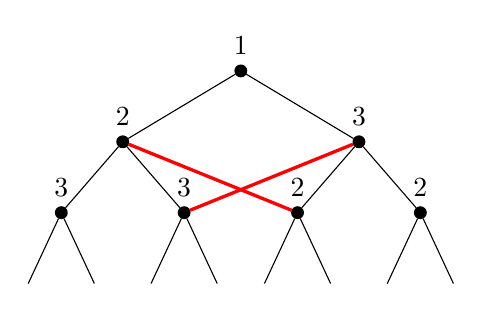
\begin{tikzpicture}[scale=0.6]
    % Node styles
    \tikzset{solid node/.style={circle,draw,fill=black,inner sep=1.5pt}}
    
    % --- Level 0: Root (Player 1) ---
    \node[solid node, label=above:1] (root) at (0, 0) {};
    
    % --- Level 1: Two nodes (Player 2 and Player 3) ---
    \node[solid node, label=above:2] (n1_left) at (-2.5, -1.5) {};
    \node[solid node, label=above:3] (n1_right) at (2.5, -1.5) {};
    
    % Edges from root
    \draw (root) -- (n1_left);
    \draw (root) -- (n1_right);
    
    % --- Level 2: Four nodes (3, 3, 2, 2) ---
    \node[solid node, label=above:3] (n2_1) at (-3.8, -3) {};
    \node[solid node, label=above:3] (n2_2) at (-1.2, -3) {};
    \node[solid node, label=above:2] (n2_3) at (1.2, -3) {};
    \node[solid node, label=above:2] (n2_4) at (3.8, -3) {};
    
    % Edges from level 1
    \draw (n1_left) -- (n2_1);
    \draw (n1_left) -- (n2_2);
    \draw (n1_right) -- (n2_3);
    \draw (n1_right) -- (n2_4);
    
    % --- Level 3: Terminals from each level 2 node ---
    % From n2_1 (first 3)
    \draw (n2_1) -- (-4.5, -4.5);
    \draw (n2_1) -- (-3.1, -4.5);
    
    % From n2_2 (second 3)
    \draw (n2_2) -- (-1.9, -4.5);
    \draw (n2_2) -- (-0.5, -4.5);
    
    % From n2_3 (first 2)
    \draw (n2_3) -- (0.5, -4.5);
    \draw (n2_3) -- (1.9, -4.5);
    
    % From n2_4 (second 2)
    \draw (n2_4) -- (3.1, -4.5);
    \draw (n2_4) -- (4.5, -4.5);
    
    % --- Information sets (red straight lines) ---
    % Connect n1_left to n2_3
    \draw[red, very thick] (n1_left) -- (n2_3);
    
    % Connect n1_right to n2_2
    \draw[red, very thick] (n1_right) -- (n2_2);
    
  \end{tikzpicture}\par
  }
  
  In this game, there is no good notion of ``timing'' or ``stages''. So the takeaway is that, the timing of players' moves is not important. What matters is the information structure, i.e., who knows what.
}


\section{Normal Form}

\defn{Game}{
  A game $G$ of $n$ players consists of the set of strategies $S_i$ and utility functions $u_i:S_1\times S_2\times \cdots \times S_n\to \RR$ for $i = 1,2,\cdots ,n$:
  \[
  G = \pr{S_1,S_2,\cdots,S_n;u_1,u_2,\cdots,u_n}\equiv \pr{S_i,u_i}_{i = 1}^n.
  \]
}

\defn{Belief}{
  A belief of player $i$, denoted by $\mu_i\in \Delta(S_{-i})$, is a probability distribution over $S_1\times \cdots\times S_{i-1}\times S_{i+1}\times \cdots\times S_n \equiv S_{-i}$.
}

\rmkb[]{
  A belief is a probability distribution over $S_{-i}$, i.e., $\mu_i\in \Delta_{-i}$. But typically,
  \[
  \Delta(S_i\times S_j)\ne \Delta(S_i)\times \Delta(S_j).
  \]
  \ex[]{
    Consider a game of 3 players where Player 2 has strategies $s_2$ and $s_2'$ to choose from, and Player 3 has $s_3$ and $s_3'$. From the Player 1's perspective, she can theoretically form the following two ``beliefs'':
    
    \begin{center}
    \begin{tabular}{c|cc}
      & $s_3$ & $s_3'$ \\
    \hline
    $s_2$ & $0$ & $1/4$ \\
    $s_2'$ & $1/4$ & $1/2$
    \end{tabular}
    \qquad
    \begin{tabular}{c|cc}
      & $s_3$ & $s_3'$ \\
    \hline
    $s_2$ & $1/9$ & $2/9$ \\
    $s_2'$ & $4/9$ & $4/9$
    \end{tabular}
    \end{center}
    Note that the first belief belongs to $\Delta(S_2\times S_3)$ but not $\Delta(S_2)\times \Delta(S_3)$, while the second belief belongs to both $\Delta(S_2\times S_3)$ and $\Delta(S_2)\times \Delta(S_3)$.
  }
}

Consider the game where Player 1 has strategy space $S_1 = \brace{s_1,s_1',s_1''}$, and Player 2 has strategy space $S_2 = \brace{s_2,s_2'}$. The normal form of this game is mapping from the strategy profiles to the payoffs of the players. In this example, it can be illustrated by a $3\times 2$ matrix:
\\

{\centering
\begin{tabular}{c|cc}
              & $s_2$ & $s_2'$ \\ \hline
            $s_1$ & $\times$ & $\times$ \\ 
            $s_1'$ & $\times$ & $\times$ \\
            $s_1''$ & $\times$ & $\times$
\end{tabular}\par
}

~\\
\rmkb[Relationship Between Game Trees and Normal Forms]{
\begin{itemize}
  \item Every tree leads to a unique normal form.
  \item However, a normal form can lead to multiple game trees that are ``equivalent''.
  
\begin{center}
    % === 第一列：左侧博弈树 (Player 1 先动) ===
    \begin{minipage}{0.35\textwidth}
        \centering
        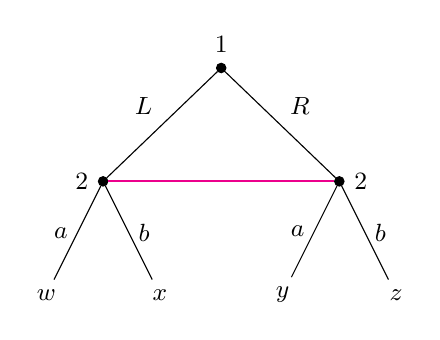
\begin{tikzpicture}[scale=1.2, font=\small]
            % 定义层级距离
            \tikzstyle{level 1}=[level distance=1.2cm, sibling distance=2.5cm]
            \tikzstyle{level 2}=[level distance=1.2cm, sibling distance=1.2cm]
            % 定义实心黑点样式 (只用于 Player 1 和 2 的决策点)
            \tikzstyle{solid node}=[circle,draw,inner sep=1.2pt,fill=black]
            
            % 树结构
            \node[solid node, label=above:{1}] (root) {}
                child {node[solid node, label=left:{2}] (n1) {}
                    % 这里将 w 和 x 直接作为节点内容，放在树枝末端
                    child {node {$w$} edge from parent node[left] {$a$}}
                    child {node {$x$} edge from parent node[right] {$b$}}
                    edge from parent node[above left] {$L$}
                }
                child {node[solid node, label=right:{2}] (n2) {}
                    % 这里将 y 和 z 直接作为节点内容
                    child {node {$y$} edge from parent node[left] {$a$}}
                    child {node {$z$} edge from parent node[right] {$b$}}
                    edge from parent node[above right] {$R$}
                };
            
            % 信息集 (紫红色线)
            \draw[magenta, thick] (n1) -- (n2);
        \end{tikzpicture}
    \end{minipage}%
    % === 第二列：中间博弈树 (Player 2 先动) ===
    \begin{minipage}{0.35\textwidth}
        \centering
        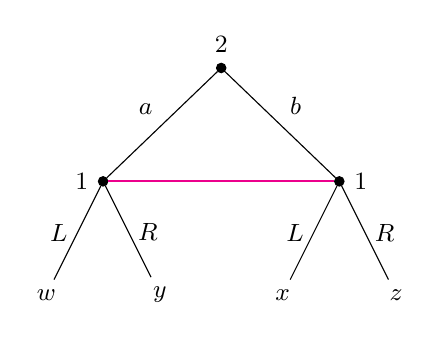
\begin{tikzpicture}[scale=1.2, font=\small]
            \tikzstyle{level 1}=[level distance=1.2cm, sibling distance=2.5cm]
            \tikzstyle{level 2}=[level distance=1.2cm, sibling distance=1.2cm]
            \tikzstyle{solid node}=[circle,draw,inner sep=1.2pt,fill=black]
            
            % 树结构
            \node[solid node, label=above:{2}] (root2) {}
                child {node[solid node, label=left:{1}] (m1) {}
                    child {node {$w$} edge from parent node[left] {$L$}}
                    child {node {$y$} edge from parent node[right] {$R$}}
                    edge from parent node[above left] {$a$}
                }
                child {node[solid node, label=right:{1}] (m2) {}
                    child {node {$x$} edge from parent node[left] {$L$}}
                    child {node {$z$} edge from parent node[right] {$R$}}
                    edge from parent node[above right] {$b$}
                };
            
            % 信息集 (紫红色线)
            \draw[magenta, thick] (m1) -- (m2);
        \end{tikzpicture}
    \end{minipage}%
    % === 第三列：右侧支付矩阵 ===
    \begin{minipage}{0.25\textwidth}
        \centering
        \renewcommand{\arraystretch}{1.5}
        \begin{tabular}{c|cc}
              & $a$ & $b$ \\ \hline
            $l$ & $w$ & $x$ \\ 
            $r$ & $y$ & $z$ \\
        \end{tabular}
    \end{minipage}
\end{center}
  
\item Many game trees can lead to the same normal form.

\begin{minipage}{0.48\textwidth}
  \centering
  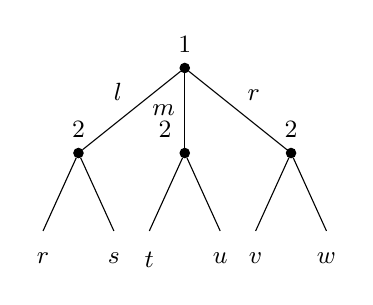
\begin{tikzpicture}[scale=0.9, font=\small]
    \tikzset{solid node/.style={circle,draw,fill=black,inner sep=1.2pt}}
    
    % Root - Player 1
    \node[solid node, label=above:1] (root) at (0, 0) {};
    
    % Level 1 - Three Player 2 nodes
    \node[solid node, label=above:2] (n1) at (-1.5, -1.2) {};
    \node[solid node, label={[xshift=-0.25cm]above:2}] (n2) at (0, -1.2) {};
    \node[solid node, label=above:2] (n3) at (1.5, -1.2) {};
    
    % Edges from root
    \draw (root) -- (n1) node[midway, above left, font=\small] {$l$};
    \draw (root) -- (n2) node[midway, left, font=\small] {$m$};
    \draw (root) -- (n3) node[midway, above right, font=\small] {$r$};
    
    % Level 2 - Outcomes
    % From n1
    \coordinate (out1) at (-2, -2.3);
    \coordinate (out2) at (-1, -2.3);
    \draw (n1) -- (out1);
    \draw (n1) -- (out2);
    
    % From n2
    \coordinate (out3) at (-0.5, -2.3);
    \coordinate (out4) at (0.5, -2.3);
    \draw (n2) -- (out3);
    \draw (n2) -- (out4);
    
    % From n3
    \coordinate (out5) at (1, -2.3);
    \coordinate (out6) at (2, -2.3);
    \draw (n3) -- (out5);
    \draw (n3) -- (out6);
    
    % Outcome labels
    \node at (out1) [below=0.15cm] {\small $r$};
    \node at (out2) [below=0.15cm] {\small $s$};
    \node at (out3) [below=0.15cm] {\small $t$};
    \node at (out4) [below=0.15cm] {\small $u$};
    \node at (out5) [below=0.15cm] {\small $v$};
    \node at (out6) [below=0.15cm] {\small $w$};
  \end{tikzpicture}
\end{minipage}%
\hspace{0.02\textwidth}
\begin{minipage}{0.48\textwidth}
  \centering
  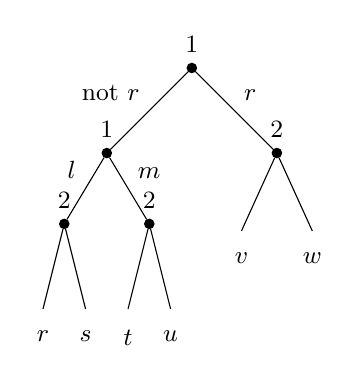
\begin{tikzpicture}[scale=0.9, font=\small]
    \tikzset{solid node/.style={circle,draw,fill=black,inner sep=1.2pt}}
    
    % Root - Player 1
    \node[solid node, label=above:1] (root) at (0, 0) {};
    
    % Level 1 - Two branches
    \node[solid node, label=above:1] (n1_left) at (-1.2, -1.2) {};
    \node[solid node, label=above:2] (n1_right) at (1.2, -1.2) {};
    
    % Edges from root
    \draw (root) -- (n1_left) node[midway, above left, font=\small] {not $r$};
    \draw (root) -- (n1_right) node[midway, above right, font=\small] {$r$};
    
    % Level 2 from left - Player 1 node has 2 branches to Player 2 nodes
    \node[solid node, label=above:2] (n2_1) at (-1.8, -2.2) {};
    \node[solid node, label=above:2] (n2_2) at (-0.6, -2.2) {};
    
    \draw (n1_left) -- (n2_1) node[midway, above left, font=\small] {$l$};
    \draw (n1_left) -- (n2_2) node[midway, above right, font=\small] {$m$};
    
    % Level 2 from right - Player 2 node with outcomes
    \coordinate (out_v) at (0.7, -2.3);
    \coordinate (out_w) at (1.7, -2.3);
    
    \draw (n1_right) -- (out_v);
    \draw (n1_right) -- (out_w);
    
    \node at (out_v) [below=0.15cm] {\small $v$};
    \node at (out_w) [below=0.15cm] {\small $w$};
    
    % Level 3 from left - outcomes
    \coordinate (out1) at (-2.1, -3.4);
    \coordinate (out2) at (-1.5, -3.4);
    \coordinate (out3) at (-0.9, -3.4);
    \coordinate (out4) at (-0.3, -3.4);
    
    % Left tree paths
    \draw (n2_1) -- (out1);
    \draw (n2_1) -- (out2);
    \draw (n2_2) -- (out3);
    \draw (n2_2) -- (out4);
    
    % Outcome labels
    \node at (out1) [below=0.15cm] {\small $r$};
    \node at (out2) [below=0.15cm] {\small $s$};
    \node at (out3) [below=0.15cm] {\small $t$};
    \node at (out4) [below=0.15cm] {\small $u$};
  \end{tikzpicture}
\end{minipage}
\end{itemize}
}

\rmk{
  Open Question: Do we lose some important information of the game by looking only at the normal form?
}

\section{Strategies}

\defn{Strategy}{
  The strategy for player $i$, denoted by $s_i$, is a complete plan of which choices to make at every one of her information sets.
}

\ex[]{
  {\centering
  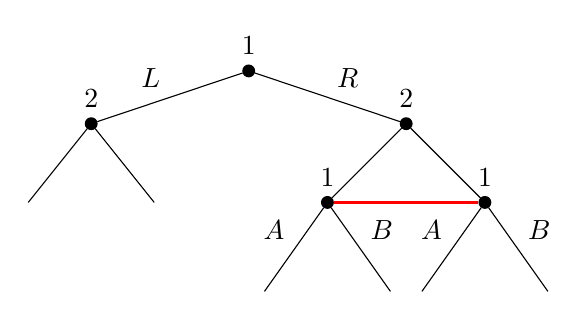
\begin{tikzpicture}[scale=1]
    % Node styles
    \tikzset{solid node/.style={circle,draw,fill=black,inner sep=1.5pt}}
    
    % --- Level 0: Root (Player 1) ---
    \node[solid node, label=above:1] (root) at (0, 0) {};
    
    % --- Level 1: Two Player 2 nodes ---
    \node[solid node, label=above:2] (n1_left) at (-2, -0.67) {};
    \node[solid node, label=above:2] (n1_right) at (2, -0.67) {};
    
    % Edges from root
    \draw (root) -- (n1_left) node[midway, above left] {$L$};
    \draw (root) -- (n1_right) node[midway, above right] {$R$};
    
    % --- Level 2: Terminal nodes from left Player 2 node ---
    \draw (n1_left) -- (-2.8, -1.67);
    \draw (n1_left) -- (-1.2, -1.67);
    
    % --- Level 2: Player 1 nodes only from right Player 2 node ---
    \node[solid node, label=above:1] (n2_left) at (1, -1.67) {};
    \node[solid node, label=above:1] (n2_right) at (3, -1.67) {};
    
    % Edge from right Player 2 node to its children
    \draw (n1_right) -- (n2_left);
    \draw (n1_right) -- (n2_right);
    
    % --- Level 3: Terminal nodes (2 from each Player 1 node) ---
    % From left Player 1 node
    \draw (n2_left) -- (0.2, -2.8) node[midway, above left] {$A$};
    \draw (n2_left) -- (1.8, -2.8) node[midway, above right] {$B$};
    
    % From right Player 1 node
    \draw (n2_right) -- (2.2, -2.8) node[midway, above left] {$A$};
    \draw (n2_right) -- (3.8, -2.8) node[midway, above right] {$B$};
    
    % --- Information set (red line connecting the two Player 1 nodes) ---
    \draw[red, very thick] (n2_left) -- (n2_right);
    
  \end{tikzpicture}\par
  }
  In this game, Player 1's strategies are $LA$, $LB$, $RA$, and $RB$, where $LA$ means that Player 1 chooses $L$ at the first information set belonging to her, and chooses $B$ at the second. The strategies at all information sets will lead to a unique outcome.
}

\rmk{
  Intuition: A player's strategy is a book with a page for each information set assigned to that player, specifying the choice there.
}

\defn{Mixed Strategy}{
  A mixed (or, randomized) strategy for player $i$, denoted by $\sigma_i$, is a probability distribution over $S_i$, i.e., $\sigma_i\in \Delta(S_i)$.
}

\rmk{
  Pure strategy is a special case of mixed strategy, with probability one choosing a specific action.
}

Rather than asking what is an optimal strategy, we think about it in a reverse way: what are the suboptimal strategies that a rational player would never choose, so that we can rule out in the analysis of equilibrium?

\defn{Strcitly Dominated Strategy (PS Notion)}{
  A pure strategy $s_i$ is strictly dominated if there is another strategy $s_i'$ such that
  \[
  u_i(s_i',s_{-i})>u_i(s_i,s_{-i}),\quad \forall s_{-i}\in S_{-i}.
  \]
}

This notion can be equivalently defined by the domination of mixed strategies.
\defn{Strictly Dominated Strategy (MS Notion)}{
  A pure strategy $s_i\in S_i$ is strictly dominated if there exists a mixed strategy $\sigma_i\in \Delta(S_i)$ such that
  \[
  u_i(\sigma_i,s_{-i})>u_i(s_i,s_{-i}),\quad \forall s_{-i}\in S_{-i},
  \]
  where $u_i(\sigma_i,s_{-i})$ is defined by
  \[
  u_i(\sigma_i,s_{-i})=\sum_{s_i'\in S_i}\sigma_i(s_i')u_i(s_i',s_{-i}).
  \]
}

\defn{Best Response}{
  A pure strategy $s_i$ is a best response to the belief $\mu_i$ if 
  \[
  u_i(s_i\mu_i)\ge u_i(s_i',\mu_i),\quad \forall s_i'\in S_i,
  \]
  where $u_i(s_i,\mu_i)$ is defined by
  \[
  u_i(s_i,\mu_i) = \sum_{s_{-i}\in S_{-i}}u_i(s_i,s_{-i})\mu_i(s_{-i}).
  \]
}

\defn{Never A Best Response (NBR)}{
  A pure strategy $s_i$ is never a best response if for all beliefs $\mu_i\in \Delta(S_{-i})$, there exists another pure strategy $s_i'\in S_i$ such that
  \[
  u_i(s_i',\mu_i)>u_i(s_i,\mu_i).
  \]
}

\thm{}{
  $s_i$ is never a best response $\iff$ $s_i$ is strictly dominated.
}

Therefore, the two notions of inferior or suboptimal strategies are equivalent. We can revisit the concept of dominated strategies from the perspective of beliefs.

\defn{Strictly Dominated Strategy (Belief Notion)}{
  A pure strategy $s_i$ is strictly dominated if there exists another pure strategy $s_i'\in S_i$ such that 
  \[
  u_i(s_i',\mu_i)>u_i(s_i,\mu_i),\quad \forall \mu_i\in \Delta(S_i).
  \]
}

\defn{Weakly Dominated Strategy (Belief Notion)}{
  A pure strategy $s_i$ is weakly dominated if there exists another pure strategy $s_i'\in S_i$ such that
  \[
  u_i(s_i',\mu_i)\ge u_i(s_i,\mu_i),\quad \forall \mu_i\in \Delta(S_i),
  \]
  and there exists some belief $\mu_i^*\in \Delta(S_{-i})$ such that
  \[
  u_i(s_i',\mu_i^*)>u_i(s_i,\mu^*).
  \]
}

\section{Iterated Elimination of Dominated Strategies}

The previous theorem states that donimated strategy is a belief-free notion. This allows us to develop the concept of iterated elimination of dominated strategies (IESDS), which is a powerful tool to analyze games without having to worry about players' beliefs.

The strategies that survive the IESDS are called \textit{rationalizable strategies}, which are the strategies that can be rationalized by some beliefs about other players' strategies. Rationalizability is a weaker notion than Nash equilibrium, as it does not require mutual consistency of beliefs. However, it is still a useful concept to understand the strategic behavior of players in a game.

Notably, IESDS's outcome is independent of the order of elimination, which is a desirable property. This is because the set of dominated strategies is well-defined and does not depend on the sequence in which they are removed. As a result, we can confidently apply IESDS to simplify games and analyze the strategic interactions without worrying about the order of elimination. This is \textit{not} the case with \textit{IEWDS} (iterated elimination of weakly dominated strategies), where the order of elimination matters.



\ex[IEWDS and Order of Elimination]{
Consider the following 2-player game and IEWDS.
~\\

\begin{center}
\begin{tabular}{c|cc}
  & $L$ & $R$ \\
\hline
$U$ & $1,1$ & $0,0$ \\
$M$ & $1,1$ & $2,1$ \\
$D$ & $0,0$ & $2,1$
\end{tabular}
\end{center}
\begin{itemize}
  \item If Player 1 eliminates $U$ and $D$, then Player 2 can eliminate nothing, and the process ends. The survived strategies are $M$ for Player 1, and $L$ and $R$ for Player 2.
  \item If Player 1 eliminates only $U$, then Player 2 can eliminate $L$, and the process ends. The survived strategies are $M$ and $D$ for Player 1, and $R$ for Player 2.
  \item If Player 1 eliminates only $D$, then Player 2 can eliminate $R$, and the process ends. The survived strategies are $U$ and $M$ for Player 1, and $L$ for Player 2.
\end{itemize}
From this example, we can clearly see the ``outcome'' of IEWDS depends on the order of elimination.
}

